\section{Paths whose image curve is a circle}

\subsection{Unit Circle}

Unit circle is set of points in $\R^2$ defined as $C=\{(x,y)\in\mathbb{R} ^2|x^2+y^2=1\}$. Ellipse is
$C=\{(x,y)\in\mathbb{R} ^2|\frac{x^2}{a^2}+\frac{y^2}{b^2}=1\}$
Has standard parameterization of $\vec{c}(t)=\big(\cos(t),\sin(t)\big)$.\newline 

\begin{center}
    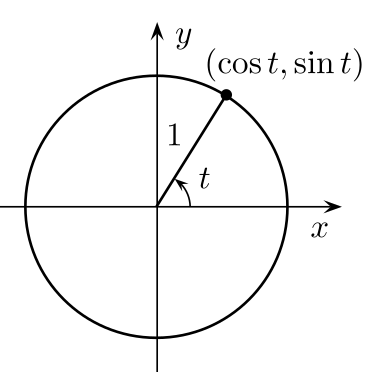
\includegraphics[scale=0.3]{unit-circle.png}
\end{center}

\noindent Properties
\begin{itemize}
    \item Image of $\vec{c}$ is a closed curve (has no endpoints, plane is divided into $\geq 2$ disjoint regions)
    \item Image of $\vec{c}$ is a simple curve; no self-intersection 
    \item $\vec{c}(t)$ is an \textbf{injective path}; path is considered injective if $\vec{c}(t_1)=\vec{c}(t_2)$, which implies that $t_1=t_2$ where 
    these are on the open interval $(a,b)$ even if $a=b$
    \item Orientation of $\vec{c}$ is counter-clockwise in traversal
\end{itemize}

\subsection{Observations}

\[\boxed{\vec{p}(t)=(a\cos (\pm nt) + x_0, b\sin (\pm nt) + y_0)}\]

If $-t$ for $t$, orientation is CW, CCW is $t$. If $a=b$, then curve is 
a circle of radius $a$ or $b$, else an ellipse with horizontal and vertical radii.
$x_0$ and $y_0$ simply shift the center coordinate. $n>0\in \R$ determines how many times
the circle is traversed given $t\in[0,2\pi]$, for example.

\section{Paths whose image is a line or line segment in the plane}

\subsection{Line Parametrics}

A line is a 1D subspace of $\R^2$, so $L=\{t\vec{m}|t\in\R\}$ for $\vec{m}\in\R^2$.
$\vec{m}=\begin{bmatrix}m_x\\m_y\end{bmatrix}$ is the \textbf{slope vector}.
Path given by image of $L$: 

\[\vec{c}(t)=\left(m_{x} t, m_{y} t\right),t\in\R\]

Can represent $\vec{c}(t)=t\vec{m}$ as well.\newline

\noindent
Lines Main Ideas
\begin{itemize}
    \item Image of a line is a curve (e.g. $y=x$ represents image curve of $\vec{c}(t)=(t,t)$)
    \item Lines can have nonzero intercepts, so $\vec{c}(t)=t\vec{m}$ represents $y=2x+1$. Line
    that has intercept vector $P_0=(x_0,y_0)$ $\parallel$ $\vec{m}=(m_x,m_y)$ can be expressed as:

    \[\boxed{\vec{c}(t)=(x_0+tm_x, y_0+m_yt)=\vec{P_0}+t\vec{m}}\]

    Note endpoint of $\vec{c}(t)$ is on image line (curve).

\end{itemize}

\subsection{General Forms}

2 parametric lines \textbf{collide} if they intersect and the point of intersection corresponds
to the same $t$ in both curves. If you set the parameter vector coordinates equal to each
other and solve for $t$, a solution indicates they collide. Intersection is found by \textbf{eliminating}
the parameter (solve for $t$ in terms of either $x$ or $y$ and plug into the other).\newline

\noindent
General form of parameterized curve can be expressed as the following:

\[\boxed{\vec{c}(t)=(\frac{m_x}{\Delta t}(t-a)+x_0,\frac{m_y}{\Delta t}(t-a)+y_0)}\]

where $\Delta t$ is the domain interval over $[a,b]$ and $(x_0,y_0)$ represents the desired \textbf{starting coordinate}.
This is important as when going in reverse, other coordinate can be used and slope might be negative.
$a$ is used in $(t-a)$ because everything is conventionally done with respect to starting coordinate.

\section{Paths whose image curve is a line in R3}

\subsection{R3 parameterization}

If $\vec{m}$ is a nonzero vector along $L$ through origin in $\R^3$, then $L=\{t\vec{m}|t\in\R\}$;
follows that $\vec{m}=(m_x,m_y,m_z)$, the slope or direction vector of the line. The basic parameterization is:

\[\vec{c}(t)=(m_x t,m_y t,m_z t)\]

Basis vectors in $\R^3$ are $\vec{i}, \vec{j}, \vec{k}$. Rewriting parameterization: 

\[\vec{c}(t)=(x_0+m_x t) \vec{i}+(y_0+m_y t) \vec{j}+(z_0+m_z t) \vec{k}\]

2 lines $\vec{c}_1(t)=P_0+\vec{m}_1t$ and $\vec{c}_2(t)=Q_0+\vec{m}_2t$ are parallel if
direction vectors are parallel ($\vec{m_1}=k\vec{m}_2$). Collisions still exist. If neither parallel nor intersecting, considered as skew.\newline

\noindent
To determine skew, parallel, or coincide, use parameters $s,t$ for each line and solve SOE.
If same slope, rule out skew clearly, then check if $s,t\in\R$: if not, then parallel, if so, then they coincide. If intersecting and want to check if collide, some $t$
must satisfy all relations.